\fancyfoot[C]{G�rel}
\section{Personenerkennung mit TensorFlow und TPU}

Die Personenerkennung mittels TensorFlow ist ein Ansatz zur Klassifizierung von Objekten und deren Kategorisierung in Echtzeit. Durch die Kombination von maschinellem Lernen, TensorFlow und spezialisierter Hardware wie TPU kann das Fahrzeug im autonomen Fahrmodus Personen erkennen und sich der Situation anpassen.
\begin{figure}[H]
    \centering
    \begin{minipage}[b]{0.45\textwidth}
        \centering
        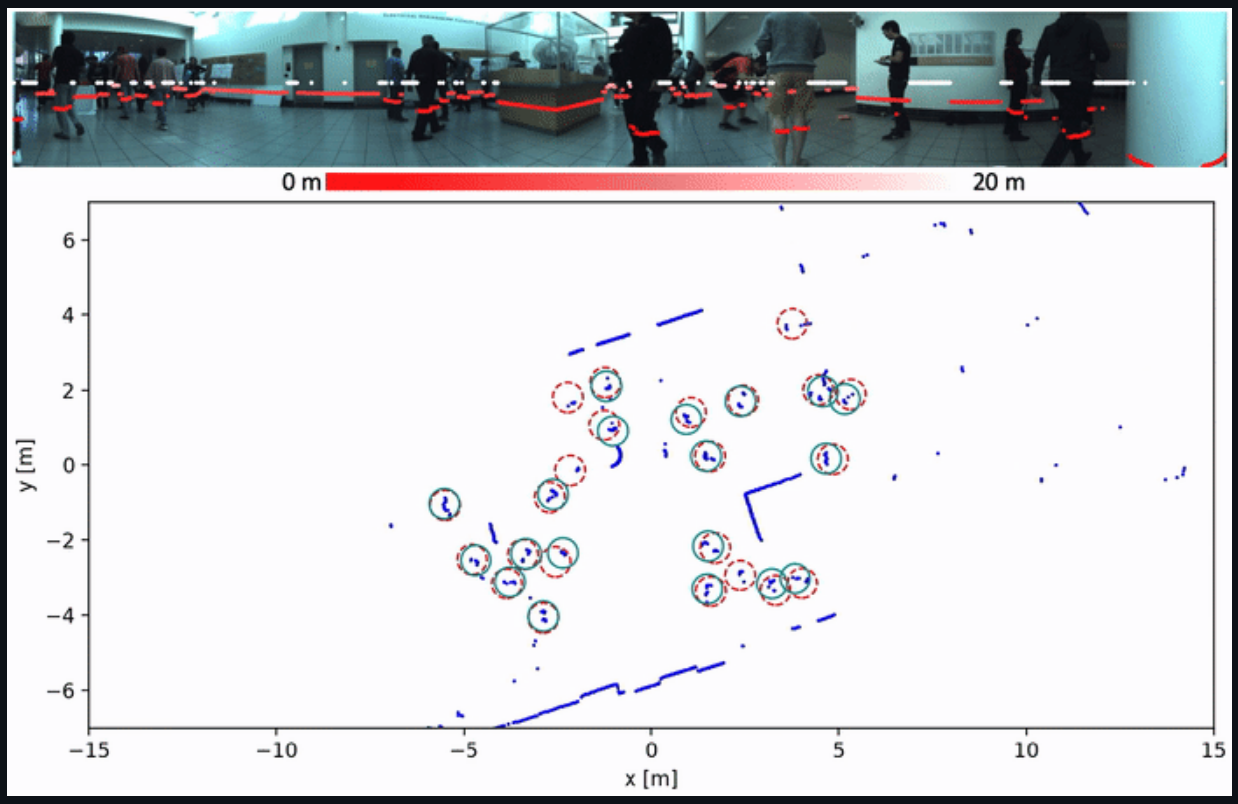
\includegraphics[scale=0.27]{./7_KI/Abbildungen/personen_erkennung_1.png}
        \caption{Symbolfoto Personenerkennung \cite{VisualComputingInstitute2021}}
    \end{minipage}
    \hfill
    \begin{minipage}[b]{0.45\textwidth}
        \centering
        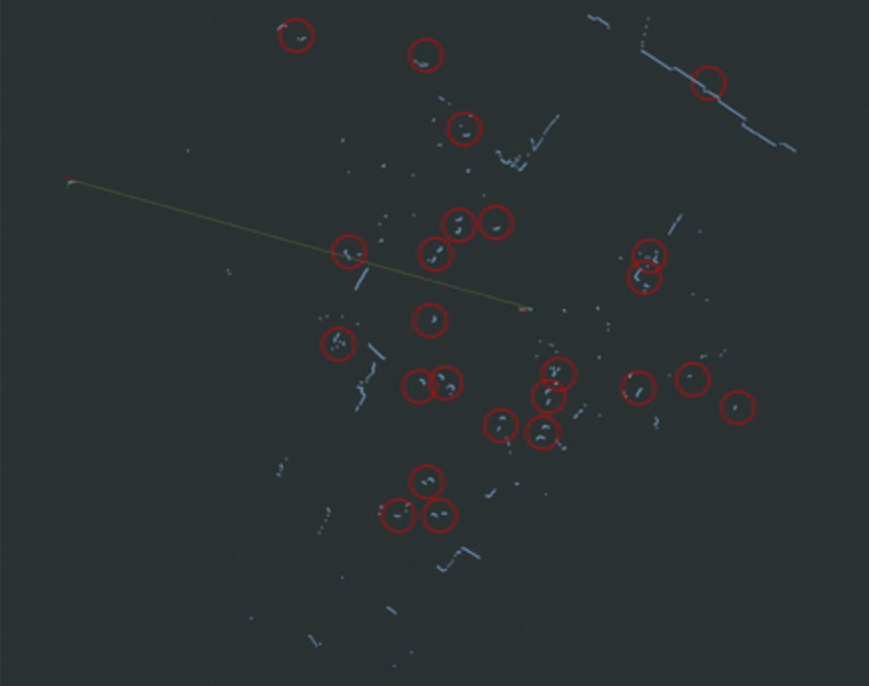
\includegraphics[scale=0.33]{./7_KI/Abbildungen/personen_erkennung_2.png}
        \caption{Symbolfoto Personenerkennung \cite{VisualComputingInstitute2021}}
    \end{minipage}
\end{figure}
\paragraph{Objekterkennung}

Die Objekterkennung ist der erste Schritt des Prozesses, bei dem die KI darauf trainiert wird, Objekte in einem Bild zu identifizieren. Durch den Einsatz von Convolutional Neural Networks (CNNs) werden Merkmale extrahiert und Muster erkannt, welche nicht der normalen Kartenumgebung entsprechen. Sobald ein Objekt erkannt wird, speichert das System die Position und das Bild des erkannten Objekts, um sp�ter darauf zugreifen zu k�nnen.

\paragraph{Objektklassifizierung}

Nachdem die Position eines erkannten Objekts gespeichert wurde, erfolgt die Klassifizierung dieses Objekts. In diesem Schritt wird die KI darauf trainiert, das erkannte Objekt richtig zu identifizieren, z. B., ob es sich um eine Person handelt oder um ein anderes Objekt. Basierend auf der Klassifizierung werden entsprechende Ma�nahmen ergriffen.

\paragraph{Bereichszuweisung und Sicherheitszonen}

Wenn das erkannte Objekt als Person klassifiziert wird, zeichnet das System eine Sicherheitszone um die gespeicherte Position der Person. Diese Zone markiert den Bereich, der f�r Fahrzeuge oder andere Objekte nicht befahren werden darf, um die Sicherheit der erkannten Personen zu gew�hrleisten. Dies ist besonders wichtig in Anwendungen wie autonomen Fahrzeugen oder Robotern, um Kollisionen zu vermeiden und sicher um Personen herum zu navigieren.

\paragraph{Training der KIs}

Ein wesentlicher Bestandteil des Prozesses ist das kontinuierliche Training der KI-Modelle. Durch die Bereitstellung von Trainingsdaten und die Verwendung von Methoden wie Transfer Learning k�nnen die Modelle verbessert und an neue Umgebungen oder Szenarien angepasst werden. Dies erm�glicht es der KI, genauere und zuverl�ssigere Ergebnisse zu liefern und sich an verschiedene Bedingungen anzupassen.